% Enable warnings about problematic code
\RequirePackage[l2tabu, orthodox]{nag}

\documentclass{WeSTassignment}

% The lecture title, e.g. "Web Information Retrieval".
\lecture{Introduction to Web Science}
% The names of the lecturer and the instructor(s)
\author{%
  Prof. Dr.~Steffen~Staab\\{\normalsize\mailto{staab@uni-koblenz.de}} \and
  Ren{\'e}~Pickhardt\\{\normalsize\mailto{rpickhardt@uni-koblenz.de}} \and
   Korok~Sengupta\\{\normalsize\mailto{koroksengupta@uni-koblenz.de}}
}
% Assignment number.
\assignmentnumber{3}
% Institute of lecture.
\institute{%
  Institute of Web Science and Technologies\\%
  Department of Computer Science\\%
  University of Luxembourg%
}
% Date until students should submit their solutions.
\datesubmission{November 16, 2016, 10:00 a.m.}
% Date on which the assignments will be discussed in the tutorial.
\datetutorial{November 18, 2016, 12:00 p.m.}

% Set langauge of text.
\setdefaultlanguage[
  variant = american, % Use American instead of Britsh English.
]{english}

% Specify bib file location.
\addbibresource{bibliography.bib}

% For left aligned centerd boxes
% see http://tex.stackexchange.com/a/25591/75225
\usepackage{varwidth}

% ==============================================================================
% Document

\begin{document}

\maketitle

The main objective of this assignment is for you understand different concepts that are associated with the "Web". In this assignment we cover two topics: 1) DNS \& 2) Internet. 

These tasks are not always specific to \enquote{Introduction to Web Science}.
For all the assignment questions that require you to write a code, make sure to include the code in the answer sheet, along with a separate python file. Where screen shots are required, please add them in the answers directly and not as separate files.\\ \\ 

%Please mention your team Names here: 
Team Name: \textbf{papa}
\\ Brigitte Aznar \\
Bonasmitha Behura \\
Ilia Tugushi

% ------------------------------------------------------------------------------

\section{DIG Deeper (5 Points)}

Assignment 1 started with you googling certain basic tools and one of them was "\emph{dig}". 
\begin{enumerate}
\item Now using that dig command, find the IP address of \url{ www.uni-koblenz-landau.de}
\item In the result, you will find "SOA". What is SOA? 
\item Copy the SOA record that you find in your answer sheet and explain each of the components of SOA with regards to your find. Merely integrating answers from the internet wont fetch you points.  

\end{enumerate}
Try the experiment once from University network and once from Home network and see if you can find any differences and if so, clarify why. 

\textbf{Answers:}\\

\begin{enumerate}
\item The IP address is 141.26.200.8 \\
\begin{figure}[h]
  \centering
  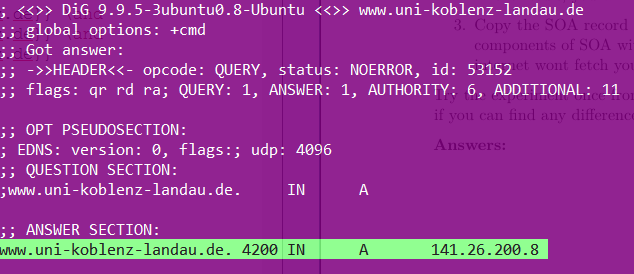
\includegraphics{dig.png}
   \caption{Dig IP address}
     \label{fig:dig} 
\end{figure}

\item SOA stands for Start of Authority, contains important information about the management of the zone, in particular zone transfer. It indicates the server(s) that are the ultimate authority for answering DNS queries about that domain.
\\ It includes
\begin{itemize}

\item The root(name) of the zone: This specifies that the zone file is for the \textbf{www.uni-koblenz-landau.de.} domain.

\item Class zone: IN (stands for Internet) 
\item SOA: indicator that this is a Start of Authority record.

\item The primary master name server for this domain: \textbf{dnsvw01.uni-koblenz-landau.de.}\\ Name servers can either be master or slaves, and if dynamic DNS is configured one server needs to be a "primary master", which goes here. If you haven't configured dynamic DNS, then this is just one of your master name servers.

\item Email address of the administrator for this zone: \textbf{root.dnsvw01.uni-koblenz-landau.de.} \\The "@" is replaced with a dot in the email address. If the name portion of the email address normally has a dot in it, this is replace with a "\textbackslash" in this part (your.name@domain.com becomes your\textbackslash name.domain.com).
\\ In this case the email would be root.dnsvw01@uni-koblenz-landau.de

\item Serial number for the zone file: \textbf{2016110401} \\Every time you edit a zone file, you must increment this number for the zone file to propagate correctly. Slave servers will check if the master server's serial number for a zone is larger than the one they have on their system. If it is, it requests the new zone file, if not, it continues serving the original file.

\item Refresh interval for the zone: \textbf{ 14400(4 hours)}\\ This is the amount of time that the slave will wait before polling the master for zone file changes.

\item Retry interval for this zone: \textbf{900(15 minutes)}\\ If the slave cannot connect to the master when the refresh period is up, it will wait this amount of time and retry to poll the master.
\item Expiry period: \textbf{604800(1 week) 900}\\ If a slave name server has not been able to contact the master for this amount of time, it no longer returns responses as an authoritative source for this zone.

\item Cache error time: \textbf{14400(4 hours)}\\This is the amount of time that the name server will cache a name error if it cannot find the requested name in this file.
\end{itemize}

\begin{figure}[!hb]
\centering
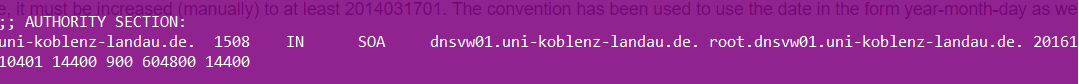
\includegraphics[scale=0.7]{soa.png}
\caption{SOA Results}
	\label{fig:soa}
\end{figure}

\end{enumerate}

% ------------------------------------------------------------------------------

\section{Exploring DNS (10 Points)}

In the first part of this assignment you were asked to develop a simple TCP Client Server. Now, using \textbf{that} client server setup.
This time a url should be send to the server and the server will split the url into the following:\\ 

\url{http://www.example.com:80/path/to/myfile.html?key1=value1&key2=value2#InTheDocument}

\begin{enumerate}
\item Protocol
\item Domain
\item Sub-Domain
\item Port number
\item Path
\item Parameters
\item Fragment
\end{enumerate}

The Protocol for sending the URL will be a string terminated with \backslash r \backslash n.

P.S.: You are \textbf{not} allowed to use libraries like \texttt{urlparse} for this question. You will also not use "Regular Expressions" for this. 

\textbf{Answer:} 

\begin{lstlisting}
import socket
import json

def Main():

    socket_server = socket.socket()
    socket_server.bind(('localhost', 8080))

    socket_server.listen(1)
    conn, addr = socket_server.accept()
    print("Connection from: " + str(addr))
    data = conn.recv(1024)
    data = data.decode('utf-8')
    if not data:
        print('no data received')
        return

    def protocol(url):
        protocol = url.split("://")
        return protocol

    def domain(url):
        domain = url.split(":")
        domain_string = domain[0].strip("www.")
        if domain_string.count(".") == 1:
            parts  = domain_string.split('.')
            domain = parts[0] + "." +parts[1] 
        elif domain_string.count(".") > 1:
            parts = domain_string.split('.')
            total = len(parts)
            domain = parts[total - 2] + "." + parts[total - 1]
        return domain

    def subdomain(url, domain):
        subdomain = url.split(domain)
        subdomain = subdomain[0].strip("www.")
        return subdomain

    def port(url):
        port = url.split(":")
        port = port[1]
        port = port.split("/")
        port = port[0]
        return port

    def path(url, port):
        path = url.split(port)
        path = path[1].split("?")
        path = path[0]
        return path 

    def params(url, path):
        params = url.split(path)
        params = params[1]
        params = params.split("#")
        params = params[0]
        return params

    def fragment(url):
        fragment = url.split("#")
        fragment = fragment[1]
        fragment = fragment.strip("\\r\\n")
        return fragment

    protocol  = protocol(data)
    url       = protocol[1]
    protocol  = protocol[0]
    domain    = domain(url)
    subdomain = subdomain(url, domain)
    port      = port(url)
    path      = path(url, port)
    params    = params(url,path)
    fragment  = fragment(url)

    print('Protocol: ', protocol)
    print('Subdomain: ', subdomain)
    print('Domain: ', domain)
    print('Port: ', port)
    print('Patha: ', path)
    print('Params: ', params)
    print('Fragments: ', fragment)
    conn.close()


if __name__ == '__main__':
    Main()
\end{lstlisting}
\begin{figure}[h]
  \centering
  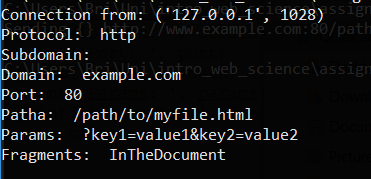
\includegraphics{splitting_url.png}
   \caption{URL parts}
     \label{fig:dig} 
\end{figure}

% ------------------------------------------------------------------------------


\section{DNS Recursive Query Resolving (5 Points)}

You have solved the "Routing Table" question in Assignment 2. We updated the routing tables once more. resulting in the following tables creating the following topology 

% Please add the following required packages to your document preamble:
% \usepackage[normalem]{ulem}
% \useunder{\uline}{\ul}{}
\begin{table}[h]
\centering
\caption{Routing Table}
\label{routing table}
\scalebox{0.8}{
\begin{tabular}{|c|c|c|c|c|c|c|c|c|c|c|}
\hline
\multicolumn{3}{|c|}{\textbf{Router1}} &        & \multicolumn{3}{c|}{\textbf{Router2}} &        & \multicolumn{3}{c|}{\textbf{Router3}} \\ \hline
Destination  & Next Hop    & Interface &        & Destination & Next Hop    & Interface &        & Destination  & Next Hop   & Interface \\ \hline
67.0.0.0     & 67.68.3.1   & eth 0     &        & 205.30.7.0  & 205.30.7.1  & eth 0     &        & 205.30.7.0   & 205.30.7.2 & eth 0     \\ \hline
62.0.0.0     & 62.4.31.7   & eth 1     &        & 156.3.0.0   & 156.3.0.6   & eth 1     &        & 88.0.0.0     & 88.6.32.1  & eth 1     \\ \hline
88.0.0.0     & 88.4.32.6   & eth 2     &        & 26.0.0.0    & 26.3.2.1    & eth 2     &        & 25.0.0.0     & 25.03.1.2  & eth 2     \\ \hline
141.71.0.0   & 141.71.20.1 & eth 3     &        & 141.71.0.0  & 141.71.26.3 & eth 3     &        & 121.0.0.0    & 121.0.3.1  & eth 3     \\ \hline
26.0.0.0     & 141.71.26.3 & eth3      &        & 67.0.0.0    & 141.71.20.1 & eth 3     &        & 156.3.0.0    & 205.30.7.1 & eth 0     \\ \hline
156.3.0.0    & 88.6.32.1   & eth 2     &        & 62.0.0.0    & 141.71.20.1 & eth 3     &        & 26.0.0.0     & 205.30.7.1 & eth 0     \\ \hline
205.30.7.0   & 141.71.26.3 & eth 3     &        & 88.0.0.0    & 141.71.20.1 & eth 3     &        & 141.71.0.0   & 205.30.7.1 & eth 0     \\ \hline
25.0.0.0     & 88.6.32.1   & eth 2     &        & 25.0.0.0    & 205.30.7.2  & eth 0     &        & 67.0.0.0     & 88.4.32.6  & eth 1     \\ \hline
121.0.0.0    & 88.6.32.1   & eth 2     &        & 121.0.0.0   & 205.30.7.2  & eth 0     &        & 62.0.0.0     & 88.4.32.6  & eth 1     \\ \hline
\end{tabular}
}
\end{table}

\begin{figure}[h]
  \centering
  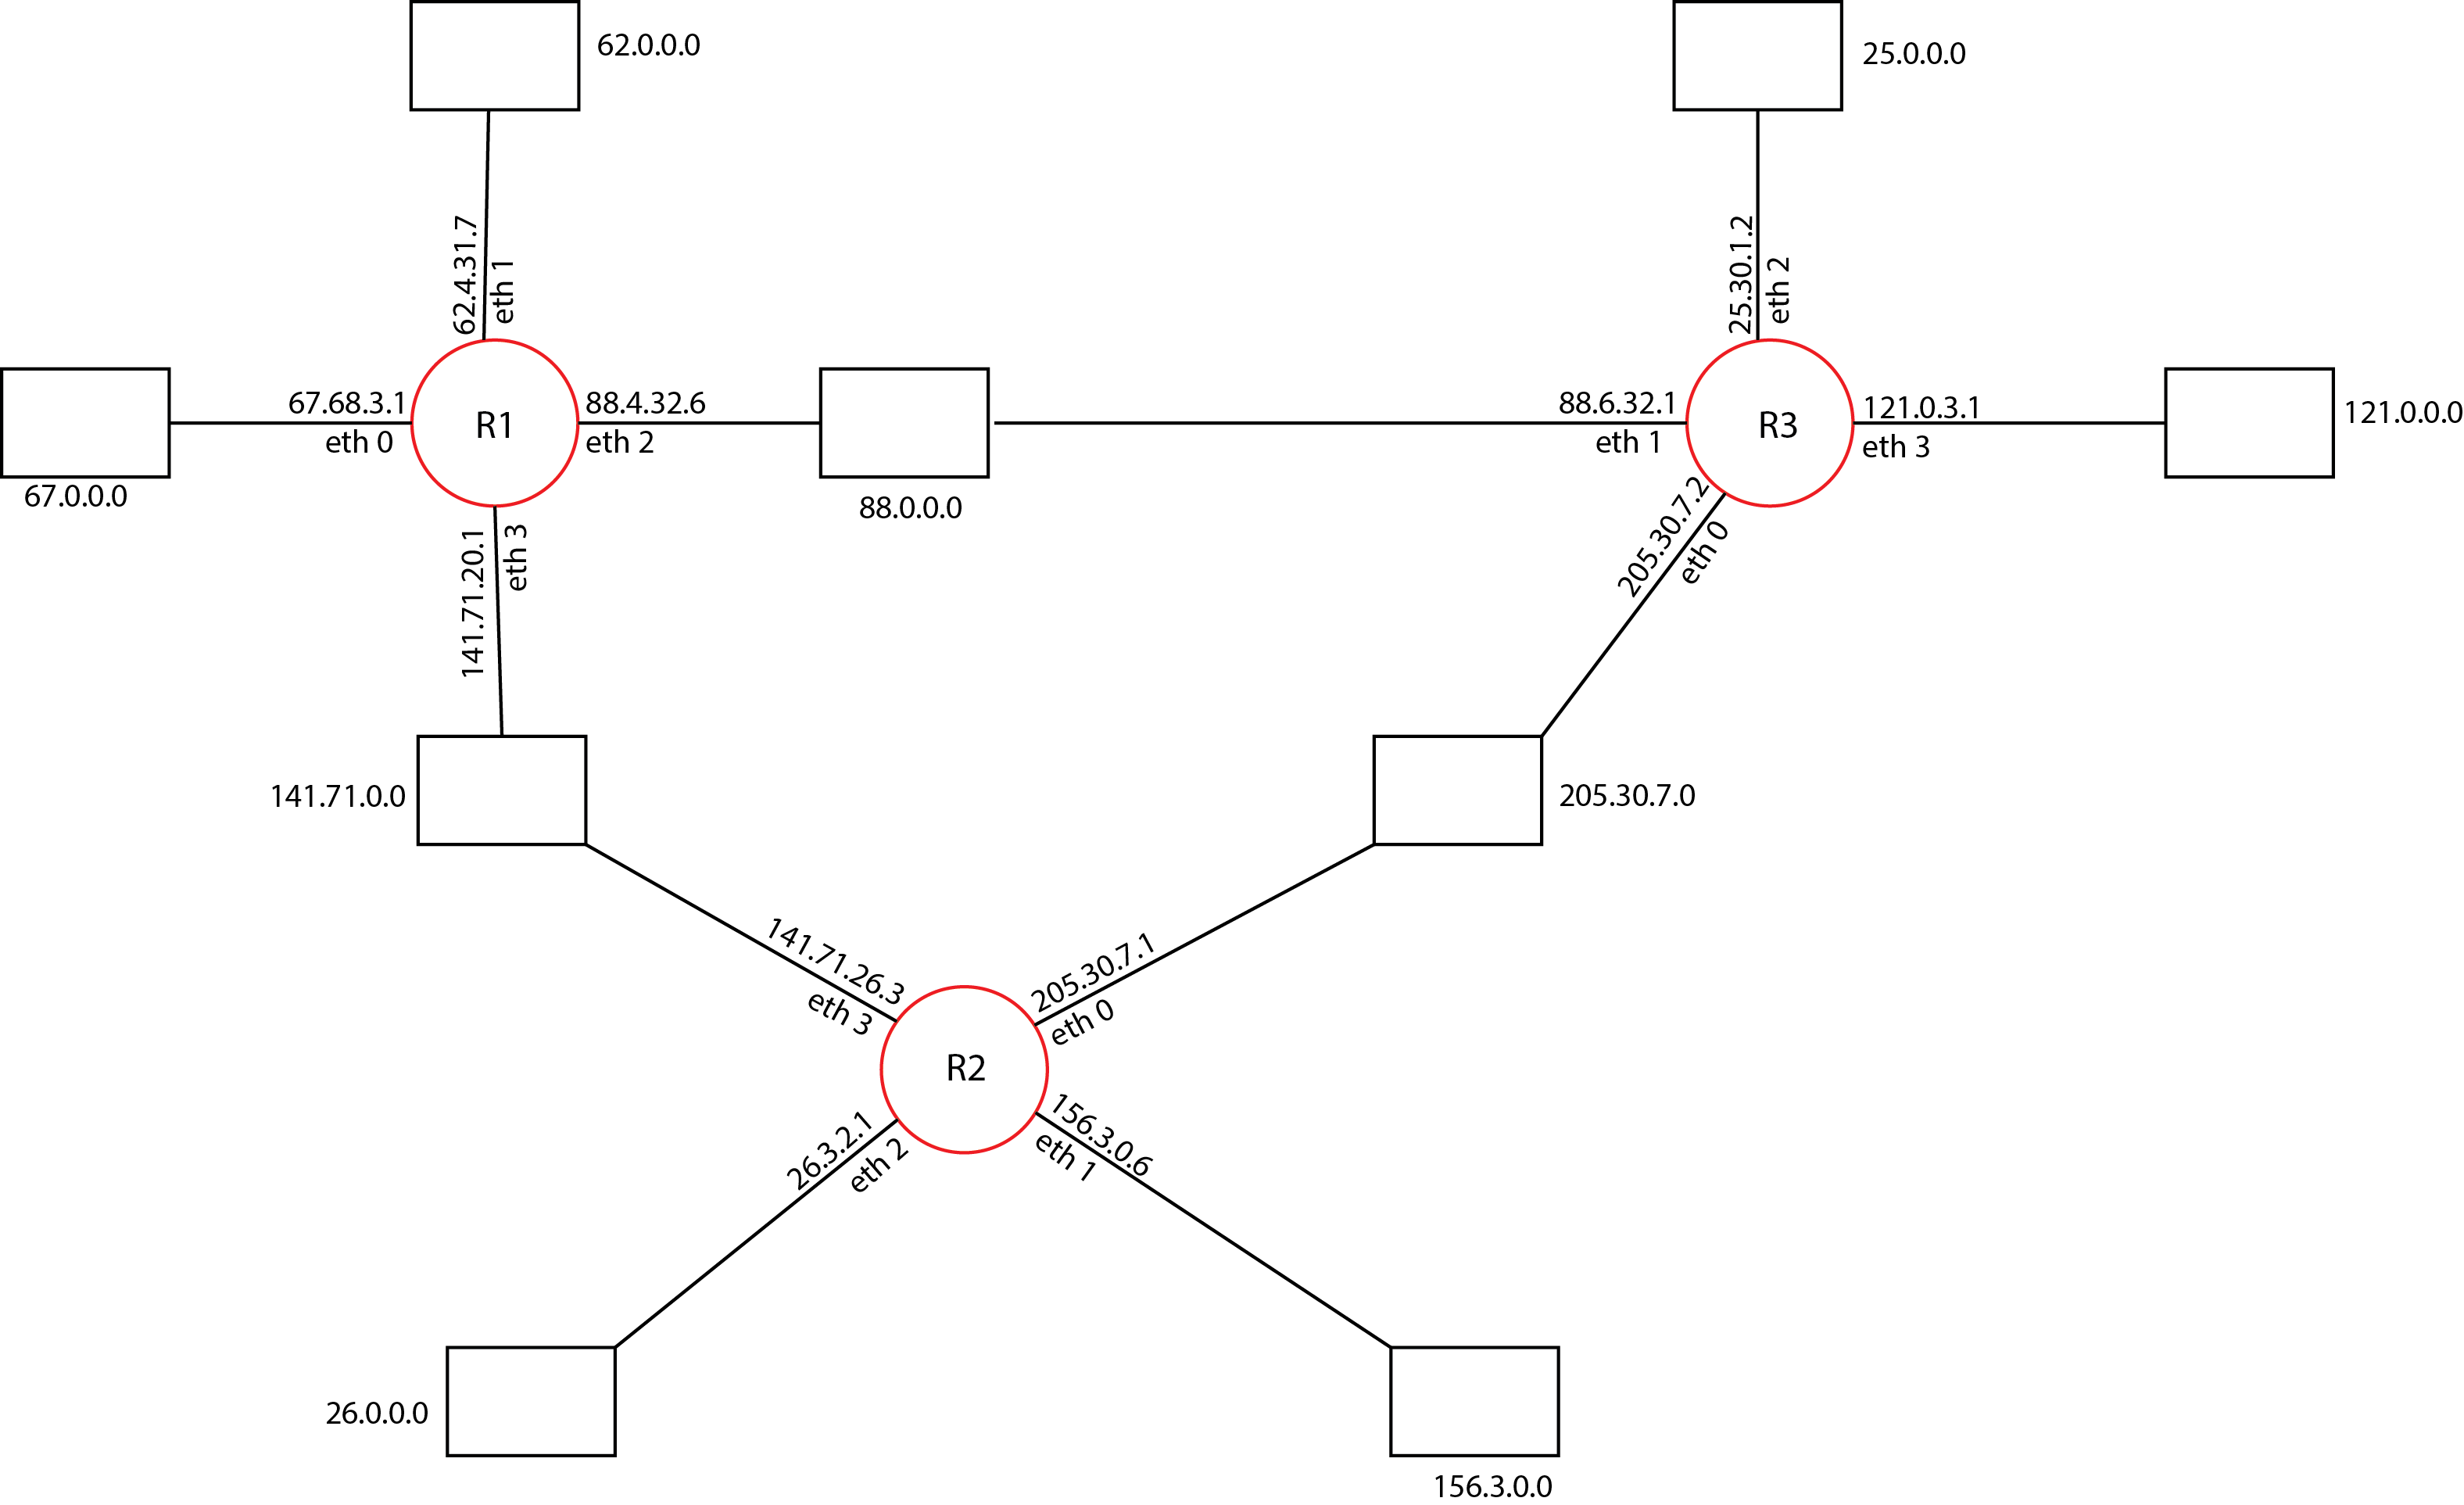
\includegraphics[scale=0.45]{ass3_DNS.png}
   \caption{DNS Routing Network}
     \label{fig:routing} 
\end{figure}

Let us asume a client with the following ip address 67.4.5.2 wants to resolve the following domain  \texttt{subdomain.webscienceexampledomain.com} using the DNS.

You can further assume the root name server has the IP address of 25.8.2.1 and the name-server for \texttt{webscienceexampledomain.com} has the IP address 156.3.20.2. 
Finally the sub-domain is handled by a name server with the IP of 26.155.36.7. 

Please explain how the traffic flows through the network in order to resolve the recursive DNS query. You can assume ARP tables are cached so that no ARP-requests have to be made. 

\textbf{Hint: You can start like this}: 

67.4.5.2 creates an IP packet with the source address XXXXXX an destination address YYYYY inside there is the DNS request. This IP packet is send as an ethernet frame to ZZZZZ. 
ZZZZZ receives the frame and forwards the encapsulated IP packet to ....

Also you can assume the DNS requests and responses will fit inside one IP packet. You also don't have to write down the specific DNS requests and responses in hex. \\ \textbf{\\ Answer:}
\\ \\ \textbf{Assuming that the root server ALLOWS recursive DNS Queries:} 
\\ The IP packet will leave the client(\textbf{67.4.5.2}) trough Router 1(\textbf{67.68.3.1 eth 0}) then it's forwarded trough \textbf{88.4.32.6 eth 2} and gets to Router 3 via \textbf{88.6.32.1 eth 1} and finally gets forwarded to the root server(\textbf{25.8.2.1}) as an Ethernet frame that includes DNS query. Here it will start recursive DNS queries to check where \texttt{subdomain.webscienceexampledomain.com} is.

So now root server will send a packet, just like the client did before. But this time to \texttt{webscienceexampledomain.com} (\textbf{156.3.20.2}) which is a known domain to it. The packet goes trough Routers 3 and 2, since it doesn't know the address for it's subdomains. Now 156.3.20.2 replies with the subdomain's IP address.

At this point the root server sends another packet to the given IP address \textbf{26.155.36.7}, this packet is sent again via Routers 3 and 2 to the IP address of the subdomain and finally it replies with the IP of the requested address.

Now the root knows the IP address, caches it and sends the requested IP Address to the client.

% ------------------------------------------------------------------------------




\makefooter

\end{document}
